\section{Solução desenvolvida}\label{sec:solucao-desenvolvida}
\textcolor{red}{retomar aqui o objetio do trabalho}
Nesta seção é discutido a solução proposta. A Figura \ref{fig:visao-geral} apresenta uma visão geral da solução.

\begin{figure*}[ht]
\centering
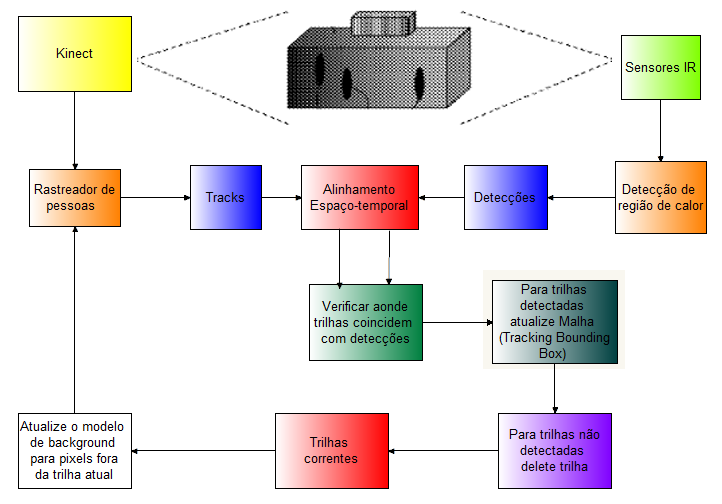
\includegraphics[width=0.8\textwidth]{images/diagrama_final.png}
\caption{Visão geral da solução proposta}
\label{fig:visao-geral}
\end{figure*}

\textcolor{red}{como dito na apresentacao, usar uma notacao mais apropriada para a figura.}

O Kinect será responsável por obter a visualização da cena de um ambiente interno. Como discutido na seção \ref{sec:trabalhos-relacionados}, o Kinect é um sensor de movimento muito eficiente, extraindo com precisão objetos, pessoas e detalhes de uma cena. 

O módulo rastreador de pessoas obtém a saída do Kinect, manipula seus dados e gera \textit{trackings}, alimentando uma base de \textit{tracks}. Essa base de tracks é consumida pelo módulo de Alinhamento espaço-temporal. 

Compondo as técnicas não visuais, serão utilizados sensores de RFID e sensores de infravermelho (\textit{Infrared - IR}). Esses são sensores precisos, eficientes e acessíveis. Os dados gerados por esses sensores serão então enviados para módulos de detecção IR e RFID. Nesses módulos serão aplicados algoritmos para detecção de pessoas.

O Componente de Alinhamento Espaço-temporal é o responsável por associar os processamentos visuais e não visuais. Nele será realizada uma verificação espaço-temporal com a finalidade de obter coincidência entre as trilhas e as detecções. Nessa análise, as trilhas que são detectadas são armazenadas na \textit{Tracking Bounding Box} que é uma malha de identificação de trilhas corretas. As trilhas que não são detectadas (não coincidem com as detecções) são então descartadas.

O Componente de Alinhamento Espaço-temporal tem como saída as trilhas corrente já validadas. Essas trilhas correntes serão utilizadas na atualização do modelo de \textit{background} servindo de retroalimentação para o módulo rastreador de pessoas.


\textcolor{red}{muito pouco, ainda que para uma proposta}

